%\chapter*{Неделя 11}
\protect\thispagestyle{fancy}
\section{}
Методом инвариантной импульсной характеристики получить цифровой аналог каскада из двух RC-цепочек интегрирующего типа. Записать разностное уравнение, передаточную функцию и построить блок-схему одной из реализаций получившегося фильтра.

\begin{figure}[!h]
	\centering
	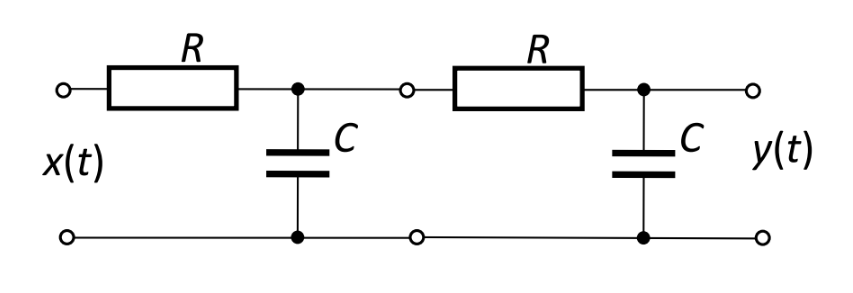
\includegraphics[width=0.55\columnwidth]{pics/fall/11/11-01.png}
	\label{fig:11-01}
\end{figure}

Уравнение для одной интегрирующей RC-цепочки:
\begin{equation*}
	RC \dfrac{dy}{dt} + y(t) = x(t).
\end{equation*}

В случае $y(0) = 0$ преобразование Лапласа принимает вид:
\begin{equation*}
	RC p \Capit{Y}(p) + \Capit{Y}(p) = \Capit{X}(p).
\end{equation*}

Передаточная функции одной RC-цепочки и каскада из двух RC-цепочек соответственно:
\begin{equation*}
	\Capit{H}_1(p) = \dfrac{\Capit{Y}(p)}{\Capit{X}(p)} = \dfrac{1}{1 + RCp},\quad
	\Capit{H}_2(p) = \big(\Capit{H}_1(p)\big)^2 = \dfrac{1}{\left(1 + RCp\right)^2}.
\end{equation*}

Вычислим обратное преобразование Лапласа:
\begin{align*}
	h_a(t) &= \dfrac{1}{2 \pi j} \oint \limits_{\gamma} \Capit{H}_2(p) e^{pt} dp = 
	\dfrac{1}{2 \pi j} \oint \limits_{\gamma} \dfrac{e^{pt} dp}{\left(1 + RCp\right)^2} = 
	\underset{p_p = -1/RC}{\text{res}} \left\{\dfrac{e^{pt}}{(1 + RCp)^2}\right\} =\\ &=
	\dfrac{1}{(RC)^2}\underset{p_p = -1/RC}{\text{res}} \left\{\dfrac{e^{pt}}{\left(p - (-\frac{1}{RC})\right)^2}\right\} =
	\dfrac{1}{(RC)^2} \lim \limits_{p \to -1/RC} \left\{\dfrac{de^{pt}}{dp}\right\} =
	\dfrac{t}{(RC)^2} \exp\left(-\dfrac{t}{RC}\right).
\end{align*}

Получим импульсную характеристику цифрового фильтра:
\begin{align*}
	h[k] &= \Delta t \cdot h_a(k \Delta t) = \dfrac{k (\Delta t)^2}{(RC)^2} \exp\left(-\dfrac{k \Delta t}{RC}\right).
\end{align*}

Наконец, передаточная функция искомого цифрового фильтра:
\begin{align*}
	\Capit{H}(z) &= \sum \limits_{k=0}^{+\infty}h[k]z^{-k} = \sum \limits_{k=0}^{+\infty} \dfrac{k \Delta t^2}{(RC)^2} \exp\left(-\dfrac{k \Delta t}{RC}\right) z^{-k} = \left(\dfrac{\Delta t}{RC}\right)^2 \sum \limits_{k=0}^{+\infty} k
	\left(\exp\left(-\dfrac{\Delta t}{RC}\right) z^{-1} \right)^k = \\ &=
	\left(\dfrac{\Delta t}{RC}\right)^2 \sum \limits_{k=0}^{+\infty} k \alpha^k = 
	\left(\dfrac{\Delta t}{RC}\right)^2 \dfrac{d}{d\alpha} \left\{ \sum \limits_{k=0}^{+\infty} \alpha^k \right\} =
	\left(\dfrac{\Delta t}{RC}\right)^2 \dfrac{d}{d\alpha} \left\{\dfrac{1}{1 - \alpha} \right\} =
	\left(\dfrac{\Delta t}{RC}\right)^2 \dfrac{\alpha}{(1 - \alpha)^2} = \\ &=
	\left(\dfrac{\Delta t}{RC}\right)^2 \dfrac{\exp\left(-\dfrac{\Delta t}{RC}\right) z^{-1} }{\left(1 - \exp\left(-\dfrac{\Delta t}{RC}\right) z^{-1} \right)^2} =
	\dfrac{\left(\dfrac{\Delta t}{RC}\right)^2 \exp\left(-\dfrac{\Delta t}{RC}\right) z^{-1}}{1 - 2\exp\left(-\dfrac{\Delta t}{RC}\right) z^{-1} + \exp\left(-\dfrac{2\Delta t}{RC}\right) z^{-2}}, \quad \Big|\exp\left(-\dfrac{\Delta t}{RC}\right) z^{-1}\Big| < 1.
\end{align*}

Разностное уравнение принимает вид:
\begin{align*}
	\left(\dfrac{\Delta t}{RC}\right)^2 \exp\left(-\dfrac{\Delta t}{RC}\right) x[k-1] = y[k] - 2\exp\left(-\dfrac{\Delta t}{RC}\right) y[k-1] + \exp\left(-\dfrac{2\Delta t}{RC}\right) y[k-2],\quad y[-2] = y[-1] = 0.
\end{align*}

\begin{figure}[!h]
	\centering
	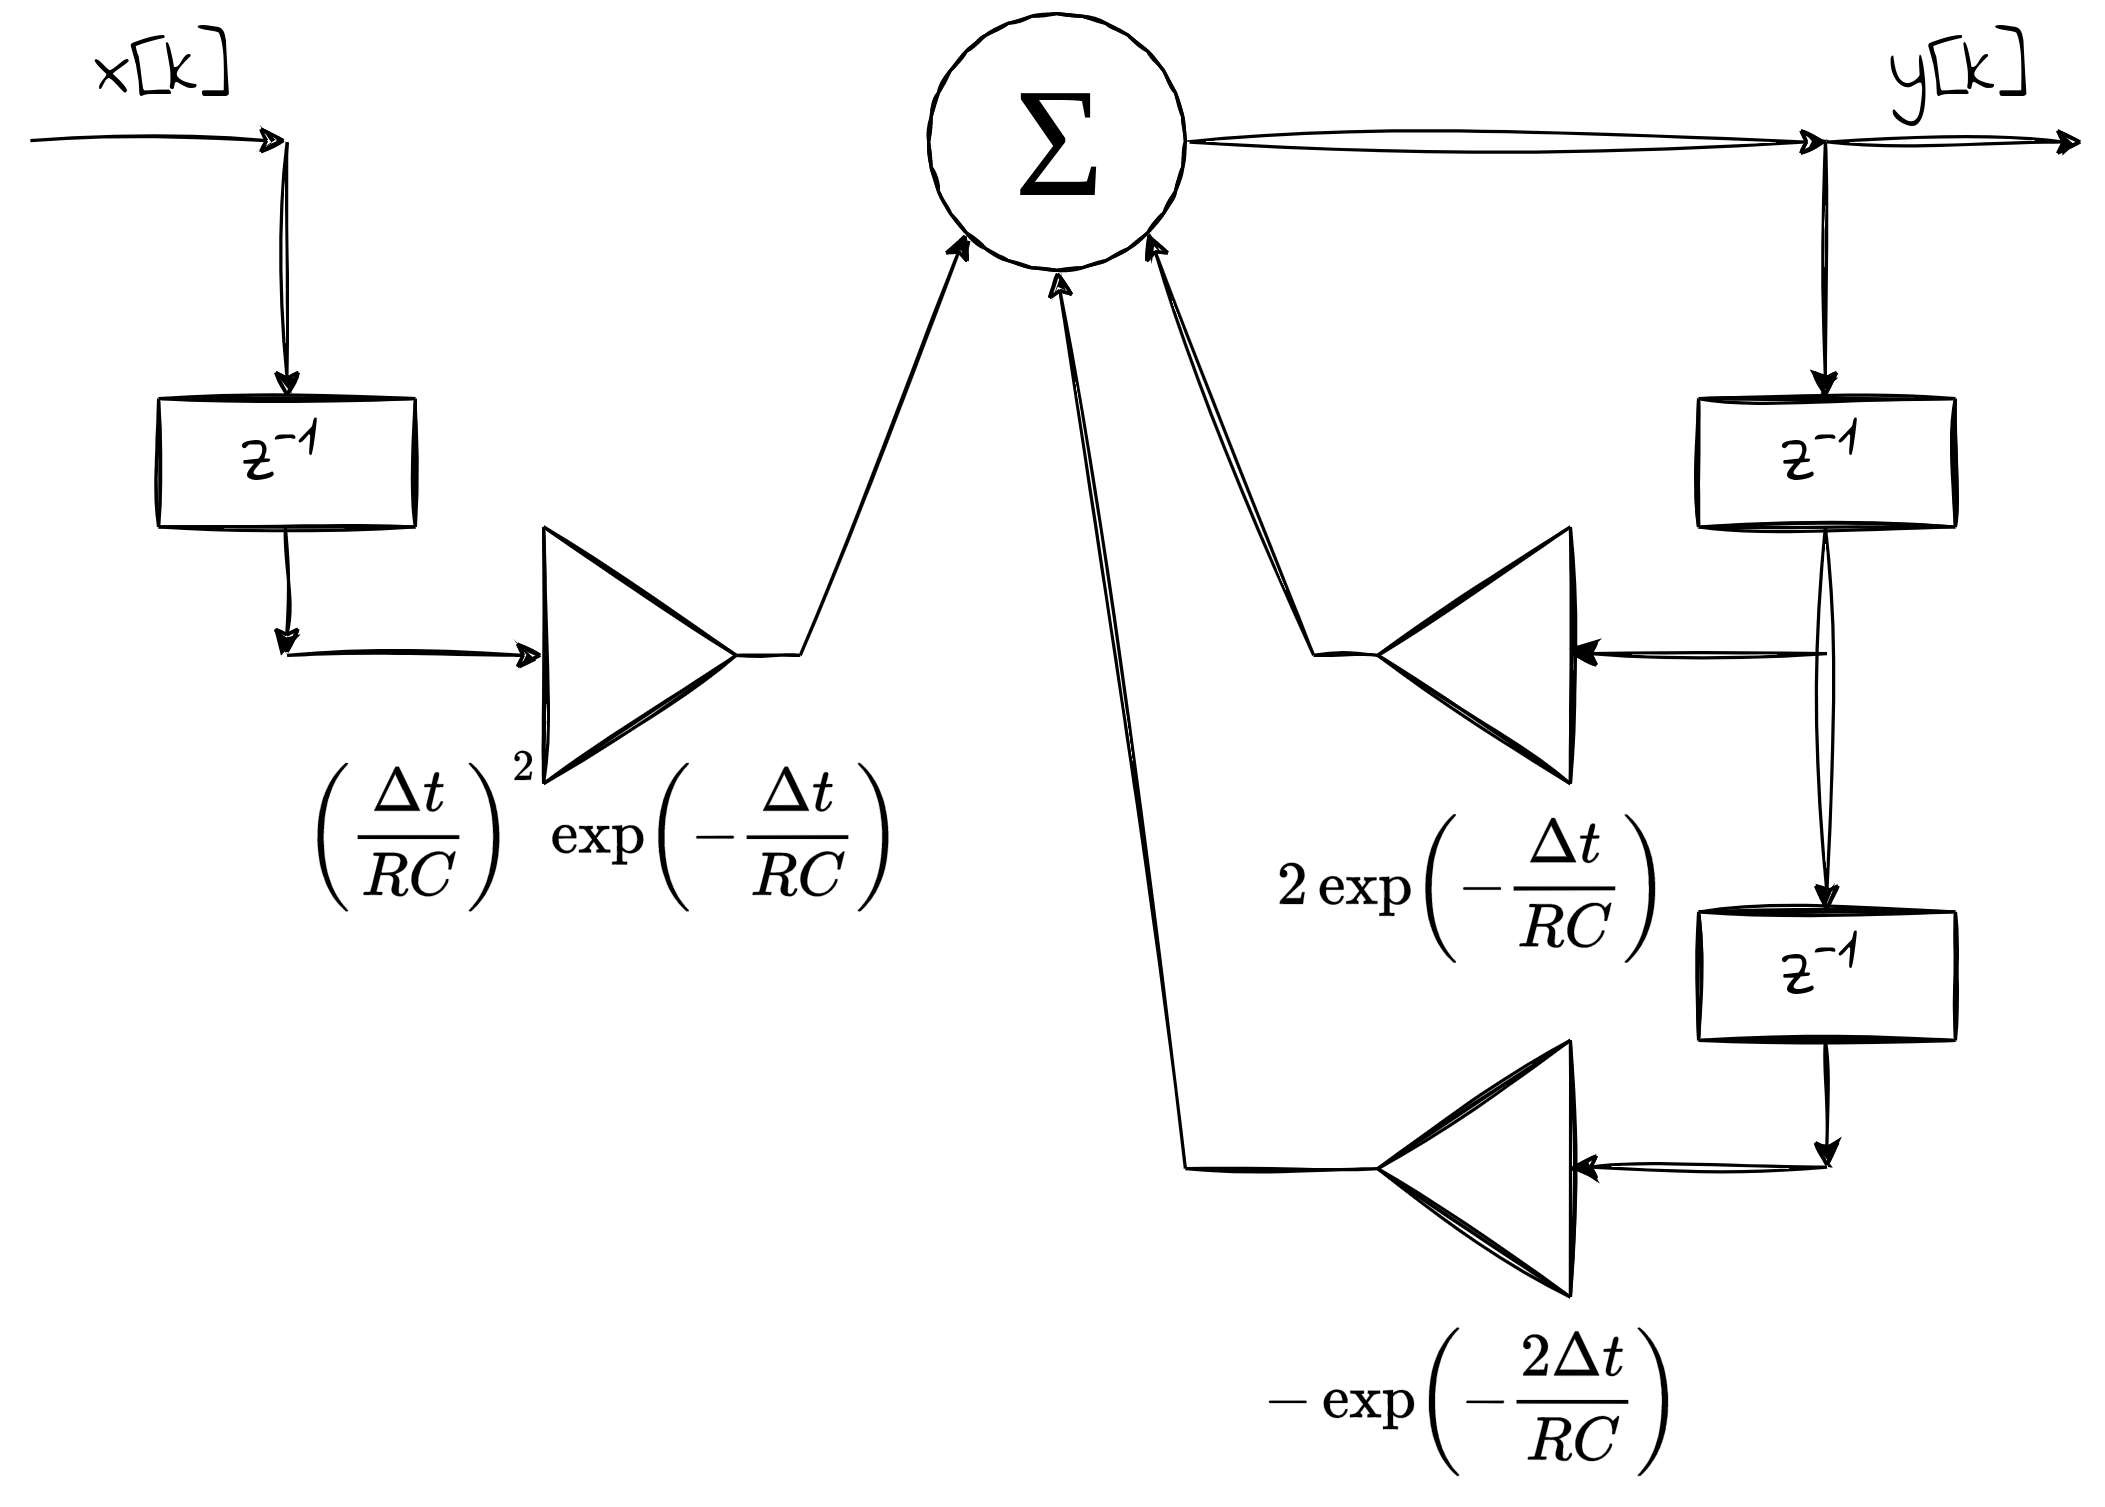
\includegraphics[width=0.75\columnwidth]{pics/fall/11/11-1.png}
	\label{fig:11-1}
\end{figure}

\newpage
\section{}
Методом билинейного $\Capit{Z}$-преобразования получить цифровой аналог RC-цепочки интегрирующего типа. Записать разностное уравнение, передаточную функцию, изобразить нуль-полюсную диаграмму и построить блок-схему одной из реализаций получившегося фильтра.

\begin{figure}[!h]
	\centering
	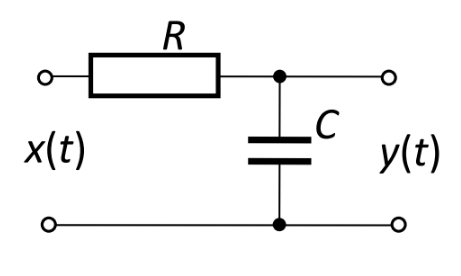
\includegraphics[width=0.35\columnwidth]{pics/fall/11/11-02.png}
	\label{fig:11-02}
\end{figure}

Уравнение для одной интегрирующей RC-цепочки:
\begin{equation*}
	RC \dfrac{dy}{dt} + y(t) = x(t).
\end{equation*}

В случае $y(0) = 0$ преобразование Лапласа принимает вид:
\begin{equation*}
	RC p \Capit{Y}(p) + \Capit{Y}(p) = \Capit{X}(p).
\end{equation*}

Передаточная функции одной интегрирующей RC-цепочки:
\begin{equation*}
	\Capit{H}_1(p) = \dfrac{\Capit{Y}(p)}{\Capit{X}(p)} = \dfrac{1}{1 + RCp}.
\end{equation*}

Согласно методу билинейного $\Capit{Z}$-преобразования делаем замену $p = \dfrac{2}{\Delta t} \dfrac{1 - z^{-1}}{1 + z^{-1}}$:

\begin{align*}
	\Capit{H}(z) = \dfrac{1}{1 + RC \dfrac{2}{\Delta t} \dfrac{1 - z^{-1}}{1 + z^{-1}}} = 
	\dfrac{1 + z^{-1}}{\left(1 + \dfrac{2RC}{\Delta t}\right) + \left(1 - \dfrac{2RC}{\Delta t}\right)z^{-1}} =
	\left( \dfrac{\Delta t}{\Delta t + 2RC}\right) \dfrac{1 + z^{-1}}{1 + \dfrac{\Delta t - 2RC}{\Delta t + 2RC}z^{-1}}.
\end{align*}


\begin{figure}[!h]
	\centering
	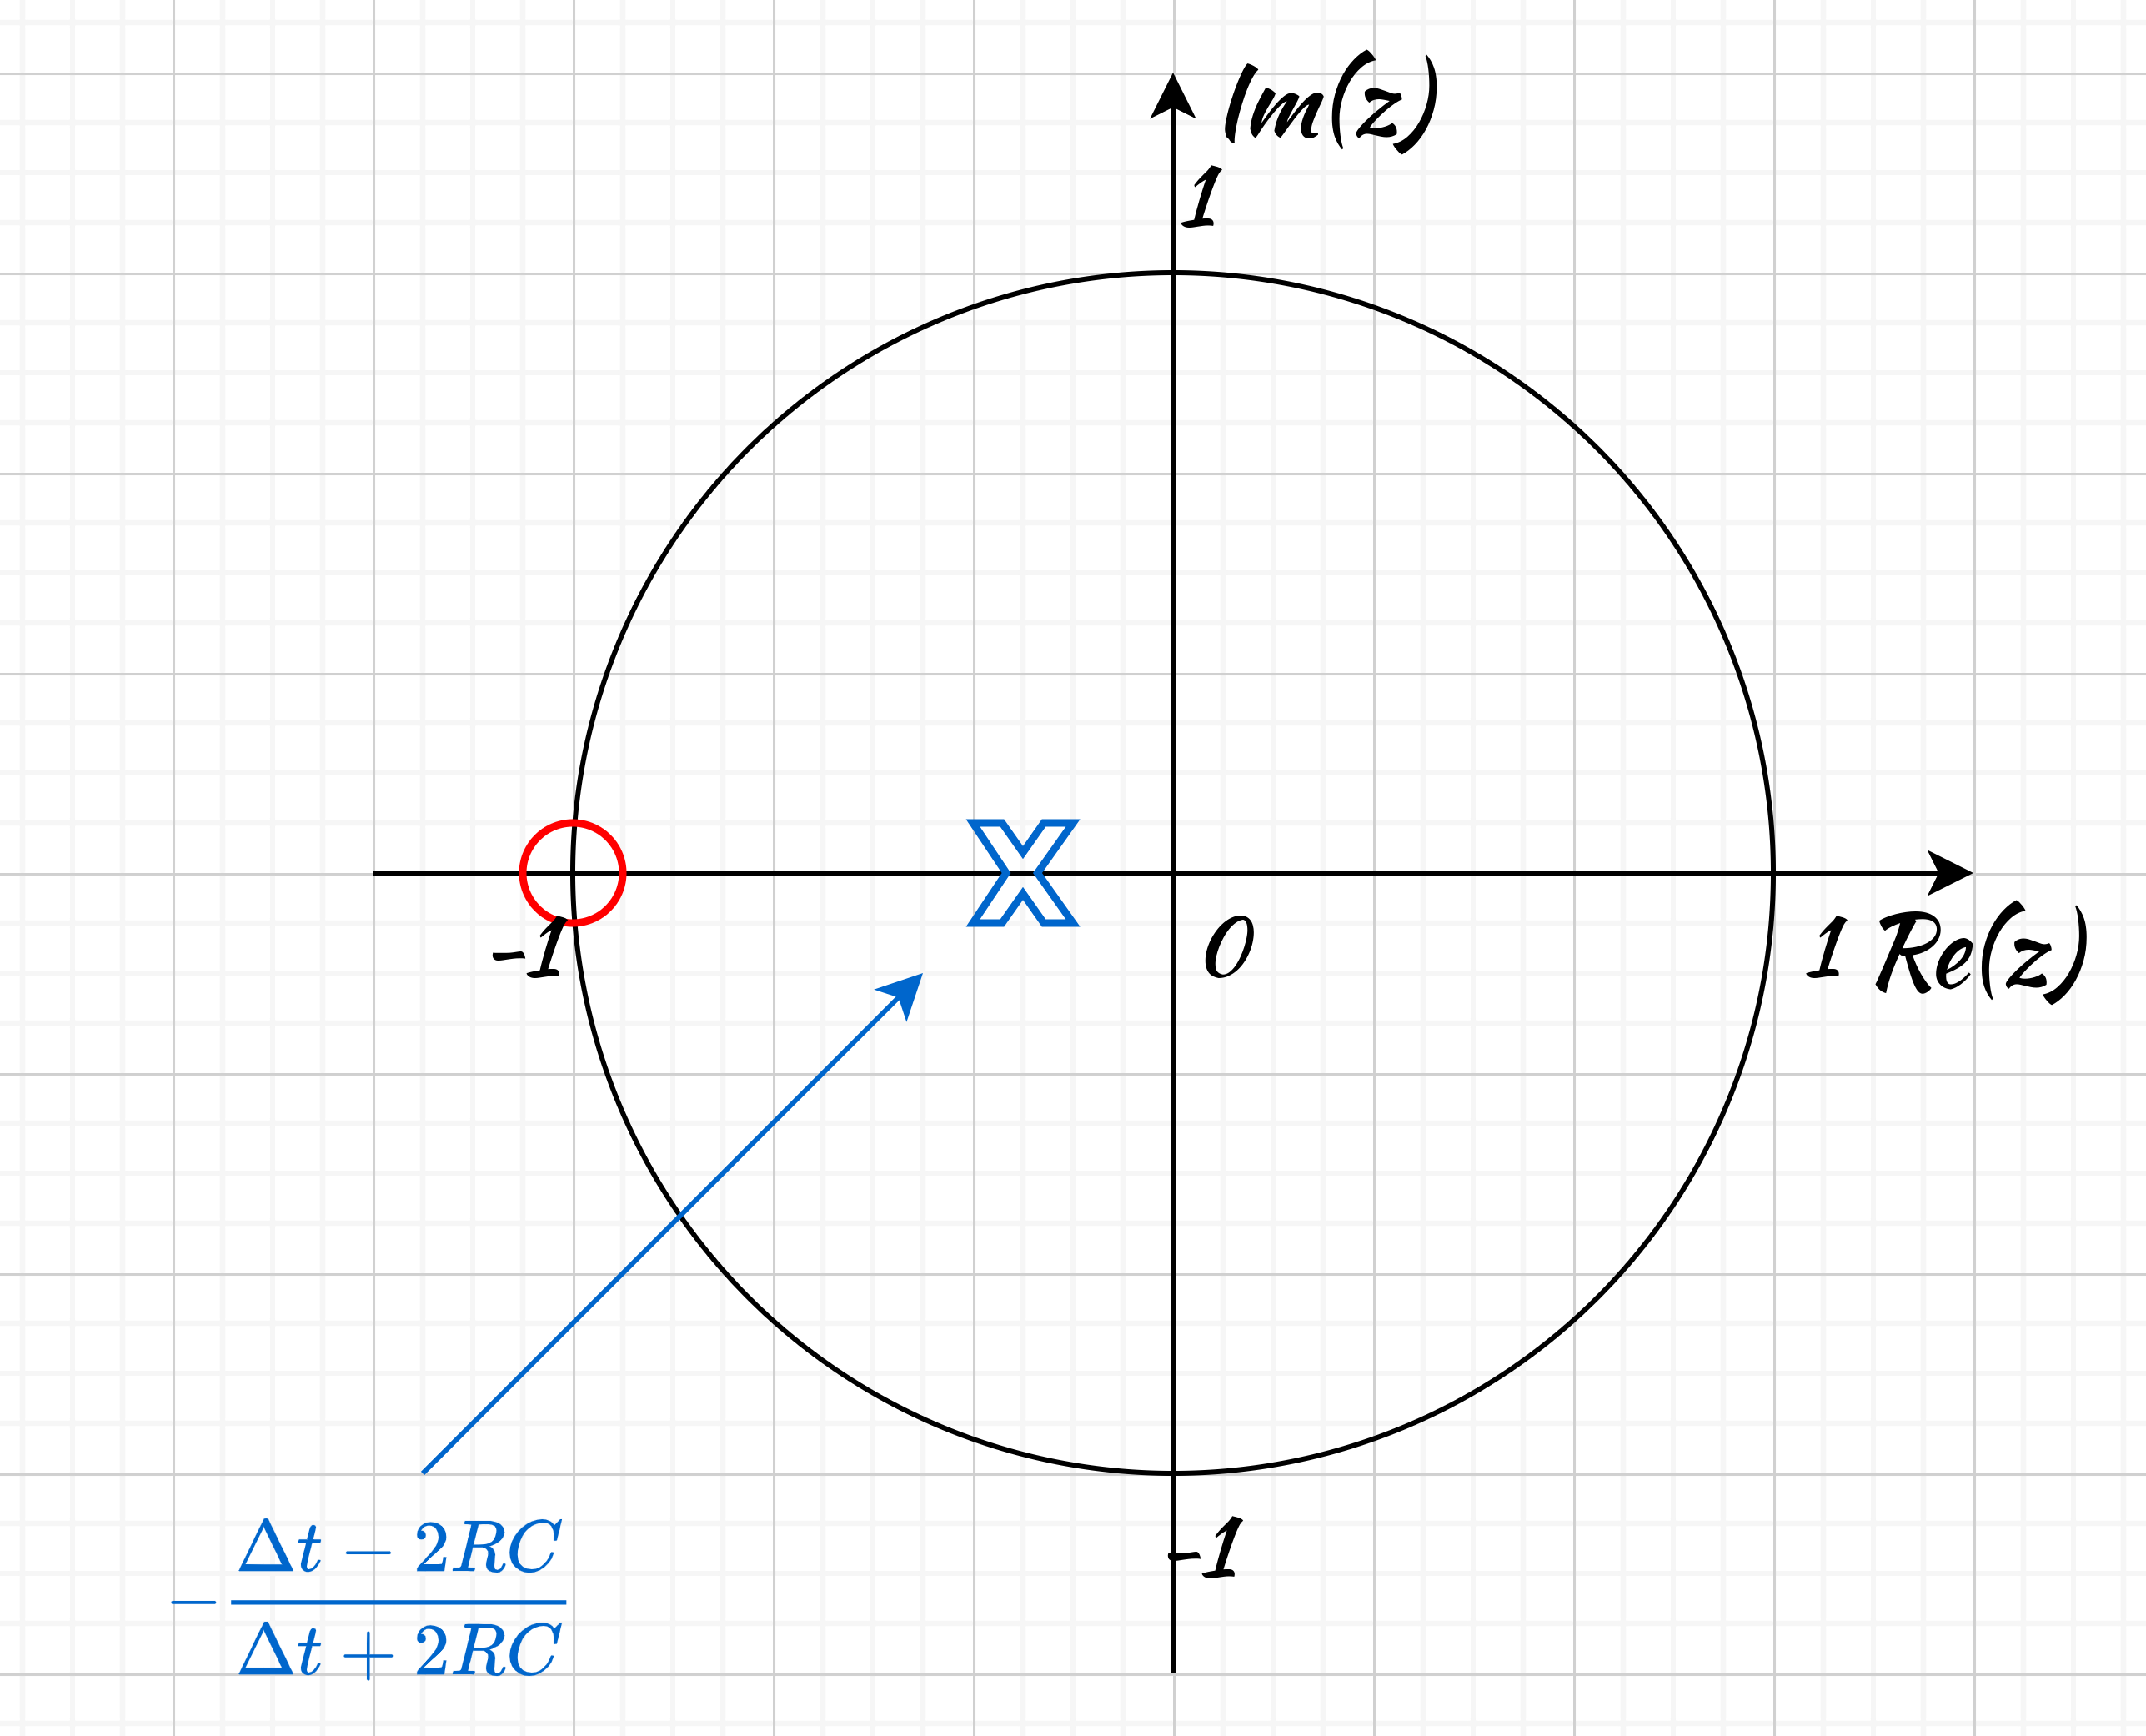
\includegraphics[width=0.55\columnwidth]{pics/fall/11/11-3.png}
	\label{fig:11-3}
\end{figure}

Разностное уравнение принимает вид:
\begin{align*}
	\left( \dfrac{\Delta t}{\Delta t + 2RC}\right) \big(x[k] + x[k-1]\big) = y[k] + \left( \dfrac{\Delta t - 2RC}{\Delta t + 2RC}\right) y[k-1], \quad y[-1] = 0.
\end{align*}


\begin{figure}[!h]
	\centering
	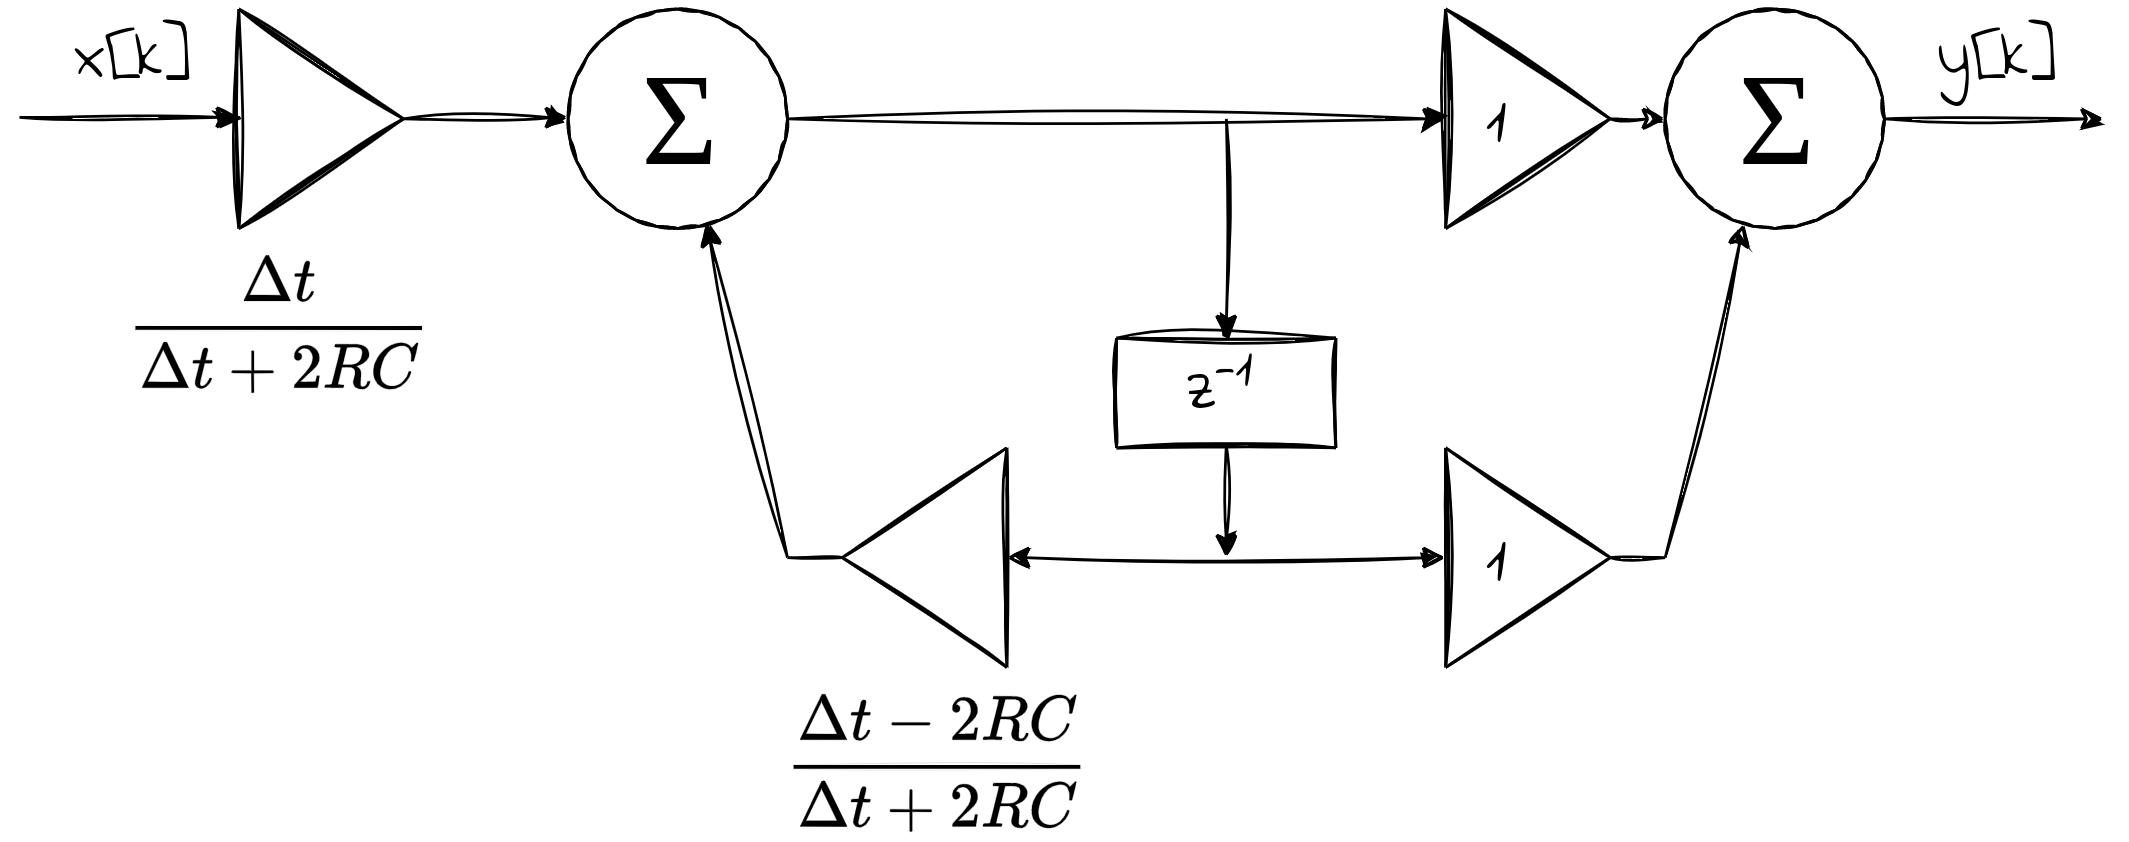
\includegraphics[width=0.75\columnwidth]{pics/fall/11/11-2.png}
	\label{fig:11-2}
\end{figure}


\newpage
\section{}
Получить выражения для частотной характеристики, АЧХ и ФЧХ фильтра, заданного разностным уравнением

\begin{equation*}
	y[k] = (1 - \Capit{A})x[k] + \Capit{A}\cdot y[k-1],\quad y[-1] = 0,
\end{equation*}
где $0 < \Capit{A} < 1$ (квазиинтегратор).



\begin{equation*}
	\Capit{H}(z) = \dfrac{\Capit{Y}(z)}{\Capit{X}(z)} = \dfrac{1 - \Capit{A}}{1 - \Capit{A}z^{-1}}
\end{equation*}

\begin{equation*}
	\Capit{H}(\nu) = \Capit{H}(z)\big|_{z = \exp(j 2\pi \nu)} = \dfrac{1 - \Capit{A}}{1 - \Capit{A}\exp(-j 2\pi \nu)} =
	\dfrac{1 - \Capit{A}}{(1 - \Capit{A}\cos(2\pi \nu)) + j \Capit{A} \sin(2\pi \nu)}.
\end{equation*}

\begin{align*}
	|\Capit{H}(\nu)| &= \dfrac{1 - \Capit{A}}{\sqrt{(1 - \Capit{A}\cos(2\pi \nu))^2 + \Capit{A}^2 \sin^2(2\pi \nu)}} = \dfrac{1 - \Capit{A}}{\sqrt{1  + \Capit{A}^2- 2\Capit{A}\cos(2\pi \nu)}}.\\
	\arg\{\Capit{H}(\nu)\} &= - \arg \{(1 - \Capit{A}\cos(2\pi \nu)) + j \Capit{A} \sin(2\pi \nu)\} =
	-\arctg \left\{ \dfrac{\Capit{A}\sin(2\pi \nu)}{1 - \Capit{A}\cos(2\pi \nu)}\right\}.
\end{align*}
